% fig_cumulative_improvement.tex
% Stacked bar chart: cumulative selectivity improvement
% TR-baseline (87L) → TR-22 (+ 87LN) → TR-23 (+ TDCS)
% Bars show: correct_baseline, gained_by_87LN, gained_by_TDCS, remaining_failure
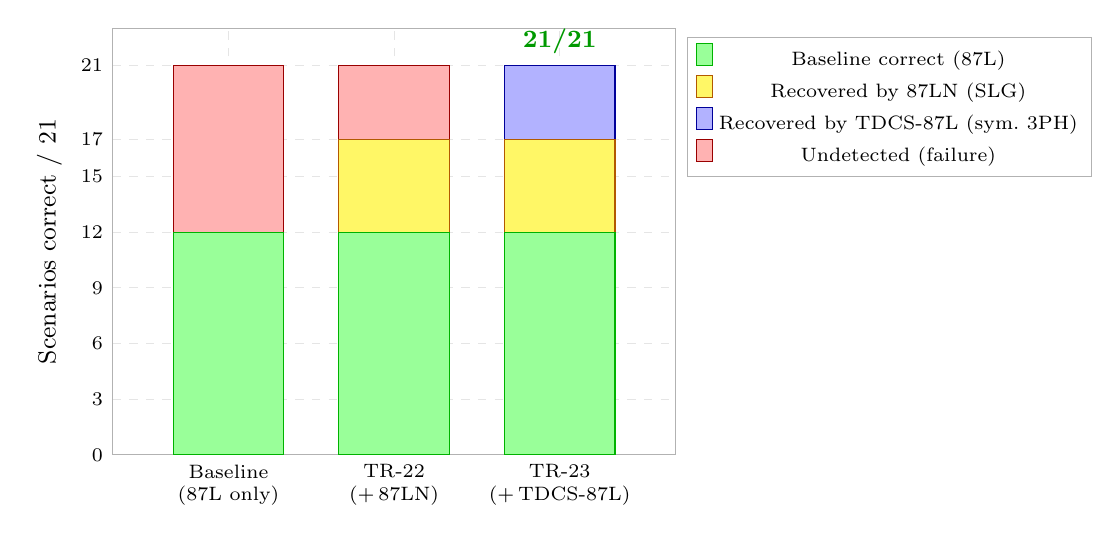
\begin{tikzpicture}
\begin{axis}[
  name         = cumax,
  ybar stacked,
  bar width    = 40pt,
  width        = 0.72\textwidth,
  height       = 7.0cm,
  ylabel       = {Scenarios correct / 21},
  ylabel style = {font=\small},
  ymin=0, ymax=23,
  ytick        = {0,3,6,9,12,15,17,21},
  yticklabels  = {0,3,6,9,12,15,17,21},
  yticklabel style={font=\scriptsize},
  xtick        = {1, 2, 3},
  xticklabels  = {Baseline\\(87L only), TR-22\\(+\,87LN), TR-23\\(+\,TDCS-87L)},
  xticklabel style={font=\scriptsize, align=center},
  enlarge x limits=0.35,
  legend style={at={(1.02,0.98)}, anchor=north west,
                font=\scriptsize, draw=gray!60},
  grid         = major,
  grid style   = {gray!20, dashed},
  tick style   = {draw=none},
  axis line style={gray!60},
]

% Correct in baseline (green): 12
\addplot[fill=green!40, draw=green!70!black]
  coordinates {(1,12) (2,12) (3,12)};
\addlegendentry{Baseline correct (87L)}

% Gained by 87LN (yellow): 0 for baseline, 5 for TR-22+
\addplot[fill=yellow!60, draw=orange!70!black]
  coordinates {(1,0) (2,5) (3,5)};
\addlegendentry{Recovered by 87LN (SLG)}

% Gained by TDCS-87L (light blue): 0, 0, 4 additional from TR-23
% (in TR-22 study: k_ibr=0.08,0.09,0.10,0.11 for 3PH = 4 cases)
% TR-23 study uses k_ibr=0.07-0.11 = 5 TDCS-only trips
% Overall improvement from 17 to 21 = 4 additional (some were already in TR-22 17)
% TR-22: SLG 7/7, 3PH 3/7, healthy 7/7 = 17/21
% TR-23 adds: 3PH 7/7, so +4 more = 21/21
\addplot[fill=blue!30, draw=blue!60!black]
  coordinates {(1,0) (2,0) (3,4)};
\addlegendentry{Recovered by TDCS-87L (sym.\ 3PH)}

% Remaining failures (red): 9, 4, 0
\addplot[fill=red!30, draw=red!60!black]
  coordinates {(1,9) (2,4) (3,0)};
\addlegendentry{Undetected (failure)}

% ---- Total labels ----------------------------------------------------------
\node[font=\small\bfseries] at (axis cs:1, 13.5) {12/21};
\node[font=\small\bfseries, orange!70!black] at (axis cs:2, 18.5) {17/21};
\node[font=\small\bfseries, green!60!black] at (axis cs:3, 22.3) {21/21};

% ---- Percentage labels -----------------------------------------------------
\node[font=\tiny] at (axis cs:1, 6.0) {57\%};
\node[font=\tiny] at (axis cs:2, 14.5) {81\%};
\node[font=\tiny, green!60!black] at (axis cs:3, 10.5) {100\%};

\end{axis}
\end{tikzpicture}
